\documentclass[parskip=full]{scrartcl}
\usepackage[top=2.54cm, bottom=2.54cm, left=2.54cm, right=2.54cm]{geometry}
\usepackage[utf8]{inputenc} % use utf8 file encoding for TeX sources
\usepackage[T1]{fontenc}    % avoid garbled Unicode text in pdf
\usepackage[ngerman]{babel}  % german hyphenation, quotes, etc
\usepackage{hyperref}       % hyperlinks in document
\usepackage{glossaries}     % glossary 
\usepackage{enumerate}      % advanced enumeration
\usepackage[shortlabels]{enumitem}
\usepackage[dvipsnames]{xcolor}
\usepackage{graphicx}
\usepackage{caption}        % add captions
\usepackage{adjustbox}      % add adjustmentbox
\usepackage{csquotes}

% Set footer and header bar
\usepackage[headsepline, footsepline]{scrlayer-scrpage}
\addtokomafont{headsepline}{\color{BlueViolet}}
\addtokomafont{footsepline}{\color{BlueViolet}}
\KOMAoptions{headsepline=1.25pt:\textwidth}
\KOMAoptions{footsepline=1.25pt:\textwidth}
\clearpairofpagestyles
\rofoot{\thepage}
\ihead{Write your own Android App: SpiceSquad}

% set the hyperlink style in the document
\hypersetup{
    pdftitle={PSE: Entwurfsheft},
    pdfborderstyle={/S/U/W 1},
    colorlinks,
    linkcolor={black!50!black},
    citecolor={blue!50!black},
    urlcolor={blue!80!black}
}

% sets right quotation for "
\MakeOuterQuote{"}

%change figure numbering
\renewcommand{\thefigure}{\thesection.\arabic{figure}}

%add command to hide subsections from toc
\newcommand{\changelocaltocdepth}[1]{%
  \addtocontents{toc}{\protect\setcounter{tocdepth}{#1}}%
  \setcounter{tocdepth}{#1}%
}

\newcommand{\enablesubsectionnumbering}[1]{
    \renewcommand{\thesubsection}{$\langle$#1\arabic{subsection}0$\rangle$}
    \changelocaltocdepth{1} 
}

\newcommand{\resetsubsectionnumbering}{
    \renewcommand{\thesubsection}{\arabic{section}.\arabic{subsection}}
    \changelocaltocdepth{3} 
}

% glossary
\makeglossaries
\renewcommand{\glossarysection}[2][]{}

\begin{document}
\newglossaryentry{label}{
    name=Label,
    plural=Labels,
    description={Rezepte können mit bezeichnenden Stichwörtern, sogenannten Labels, versehen werden. Dies ermöglicht das Filtern von Rezepten nach bestimmten Eigenschaften (z.B. vegetarisch, glutenfrei, halal)}
}

\begin{titlepage}
    \begin{center}
        \begin{Huge}
            {\textbf{Write your own Android App: SpiceSquad}}
        \end{Huge}
        \vspace{12px}

        Praxis der Softwareentwicklung (PSE)\\
        Sommersemester 2023\\
        \vspace{150px}

        \begin{Huge}
            {\textbf{Entwurfsheft}}
        \end{Huge}
        \vspace{12px}

        \textbf{Auftraggeber}\\
        Karlsruher Institut für Technologie\\
        KASTEL — Institut für Informationssicherheit und Verlässlichkeit\\
        \vspace{330px}

        \textbf{Auftragnehmer}\\
        Karlsruher Intellektuelle\\
        Henri Becker, Konrad Knappe, Lukas Schwarz, Raphael Zipperer\\
    \end{center}
\end{titlepage}

\tableofcontents
\newpage

\section*{Gender-Hinweis}
Zur besseren Lesbarkeit wird in diesem Entwurfsheft das generische Maskulinum verwendet.
Die in diesem Heft verwendeten Personenbezeichnungen beziehen sich – sofern nicht anders kenntlich gemacht – auf alle Geschlechter.


\section{Presentation layer}
    %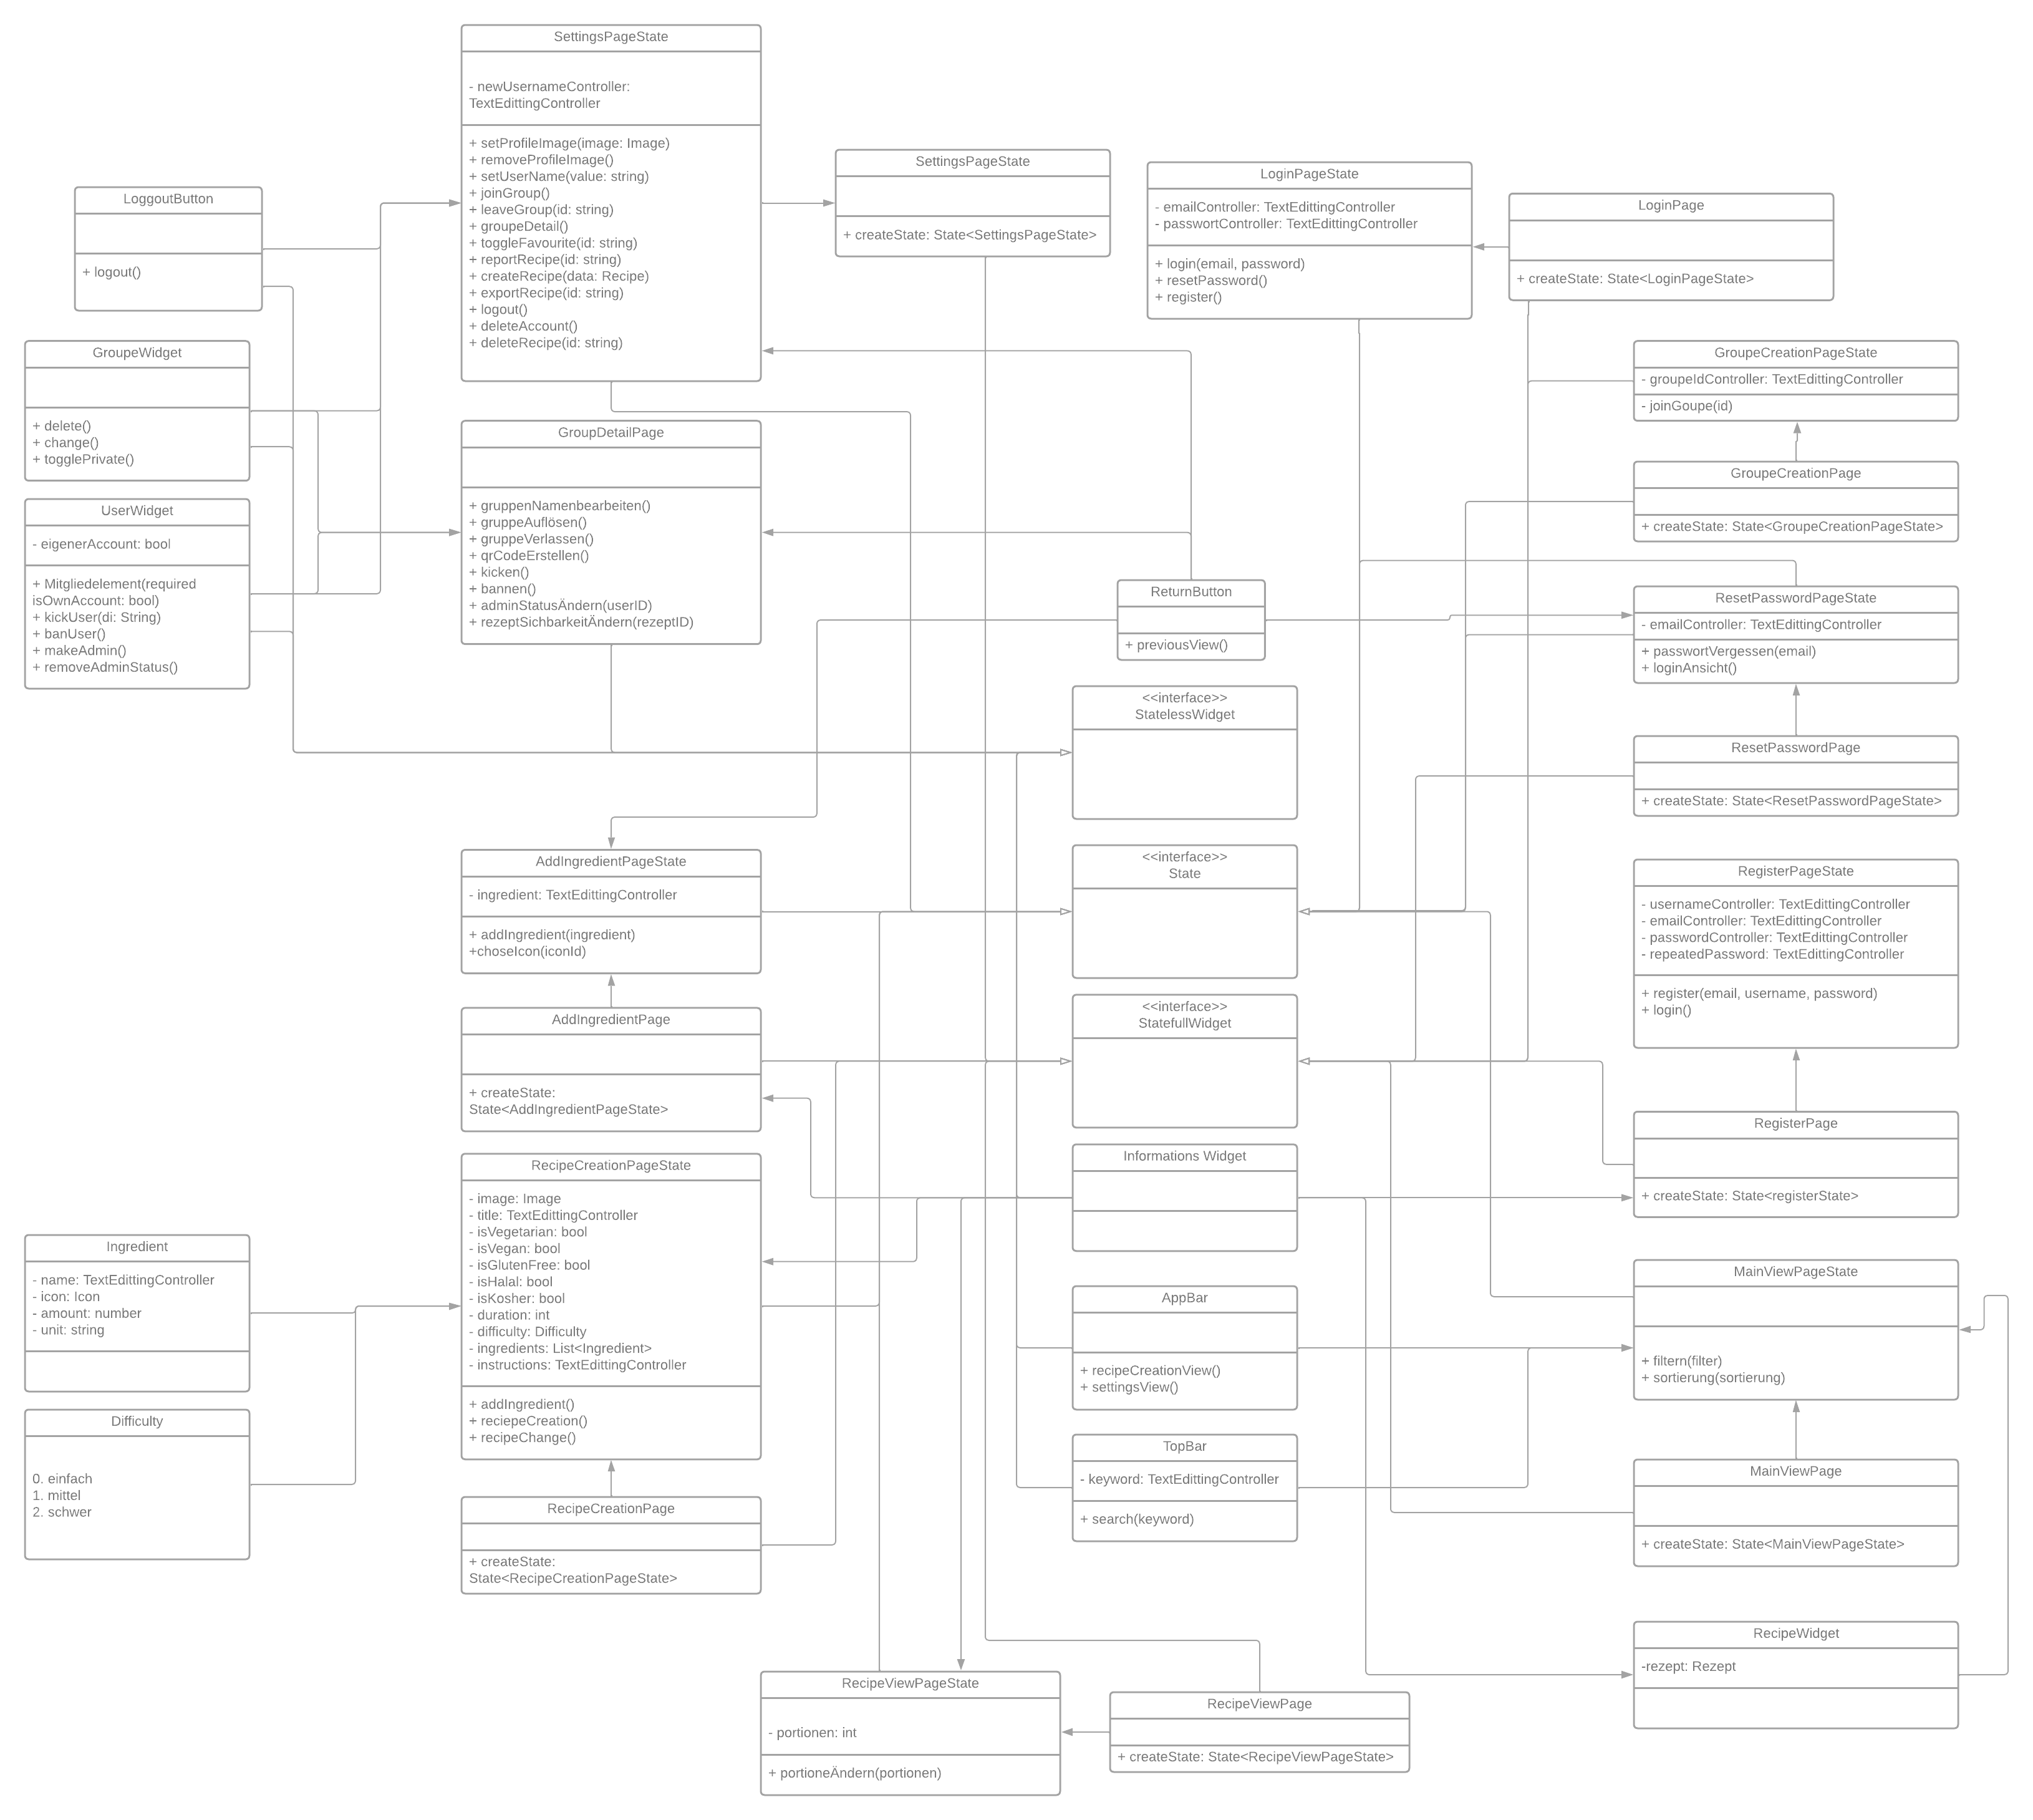
\includegraphics[width = 180mm]{entwurfsheft/images/Presentation-layer/Presentation-Layer.png}
    \newpage
    \subsection{Recipe Creation Page}
        Die Klassen beinhaltet alle nötigen Funktionen und Attribute um die Rezept-Erstell-Ansicht darzustellen.\newline
        \textbf{Attributes}
        \begin{itemize}
            \item image: Hochgeladenes Bild welches den anderen Nutzern in der Rezeptansicht angezeigt werden soll.
            \item title: Die eingegebene Zeichenkette für den Titel des Rezepts.
            \item isVegetarian: Der vom Nutzer angegebene Boolean ob das \gls{labels} Vegetarisch dem Leser angezeigt werden soll.
            \item isVegan: Der vom Nutzer angegebene Boolean ob das \gls{labels} Vegan dem Leser angezeigt werden soll.
            \item isGlutenFree: Der vom Nutzer angegebene Boolean ob das \gls{labels} Glutenfrei dem Leser angezeigt werden soll.
            \item isHalal: Der vom Nutzer angegebene Boolean ob das \gls{labels} Halal dem Leser angezeigt werden soll.
            \item isKosher: Der vom Nutzer angegebene Boolean ob das \gls{labels} Koscher dem Leser angezeigt werden soll.
            \item duration: Die vom Nutzer eingegebene Ganzzahl, welche die Zubereitunszeit in Minuten angibt.
            \item dificullty: Die vom Nutzer ausgewählte \gls{schwierigkeit} des Rezepts
            \item ingerdients: Eine Liste an Ingerdients, welche in der AddIngredientPage erstellt wurde:
            \item instructions: Die vom Nutzer angegeben Zeichenkette für die Beschreibung des Rezepts.
        \end{itemize}
        
        \textbf{Methods}
        \begin{itemize}
            \item addIngredient(): Die Page AddIngredientPage wird aufgerufen.
            \item recipeSave(): Die Methode ruft, abhängig davon ob das Rezept neu erstellt wird oder nur verändert wurde, entweder recipeCreation() oder recipeChange() auf.
        \end{itemize}

        
        %\begin{figure}[htp]
        %    \begin{minipage}
        %        [t]{0.49\textwidth}
        %        \centering
        %        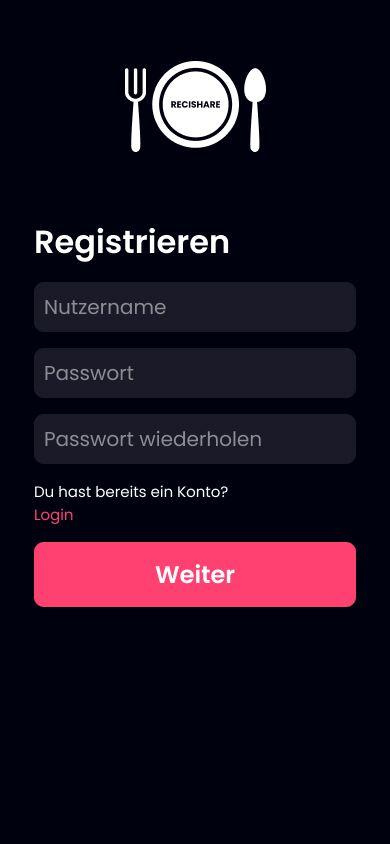
\includegraphics[height=80mm]{pflichtenheft/images/benutzeroberfläche/RegisterView.jpg}
        %        \caption{Registrierungsansicht}
        %    \end{minipage}
        %    \begin{minipage}
        %        [t]{0.49\textwidth}
        %        \centering
        %        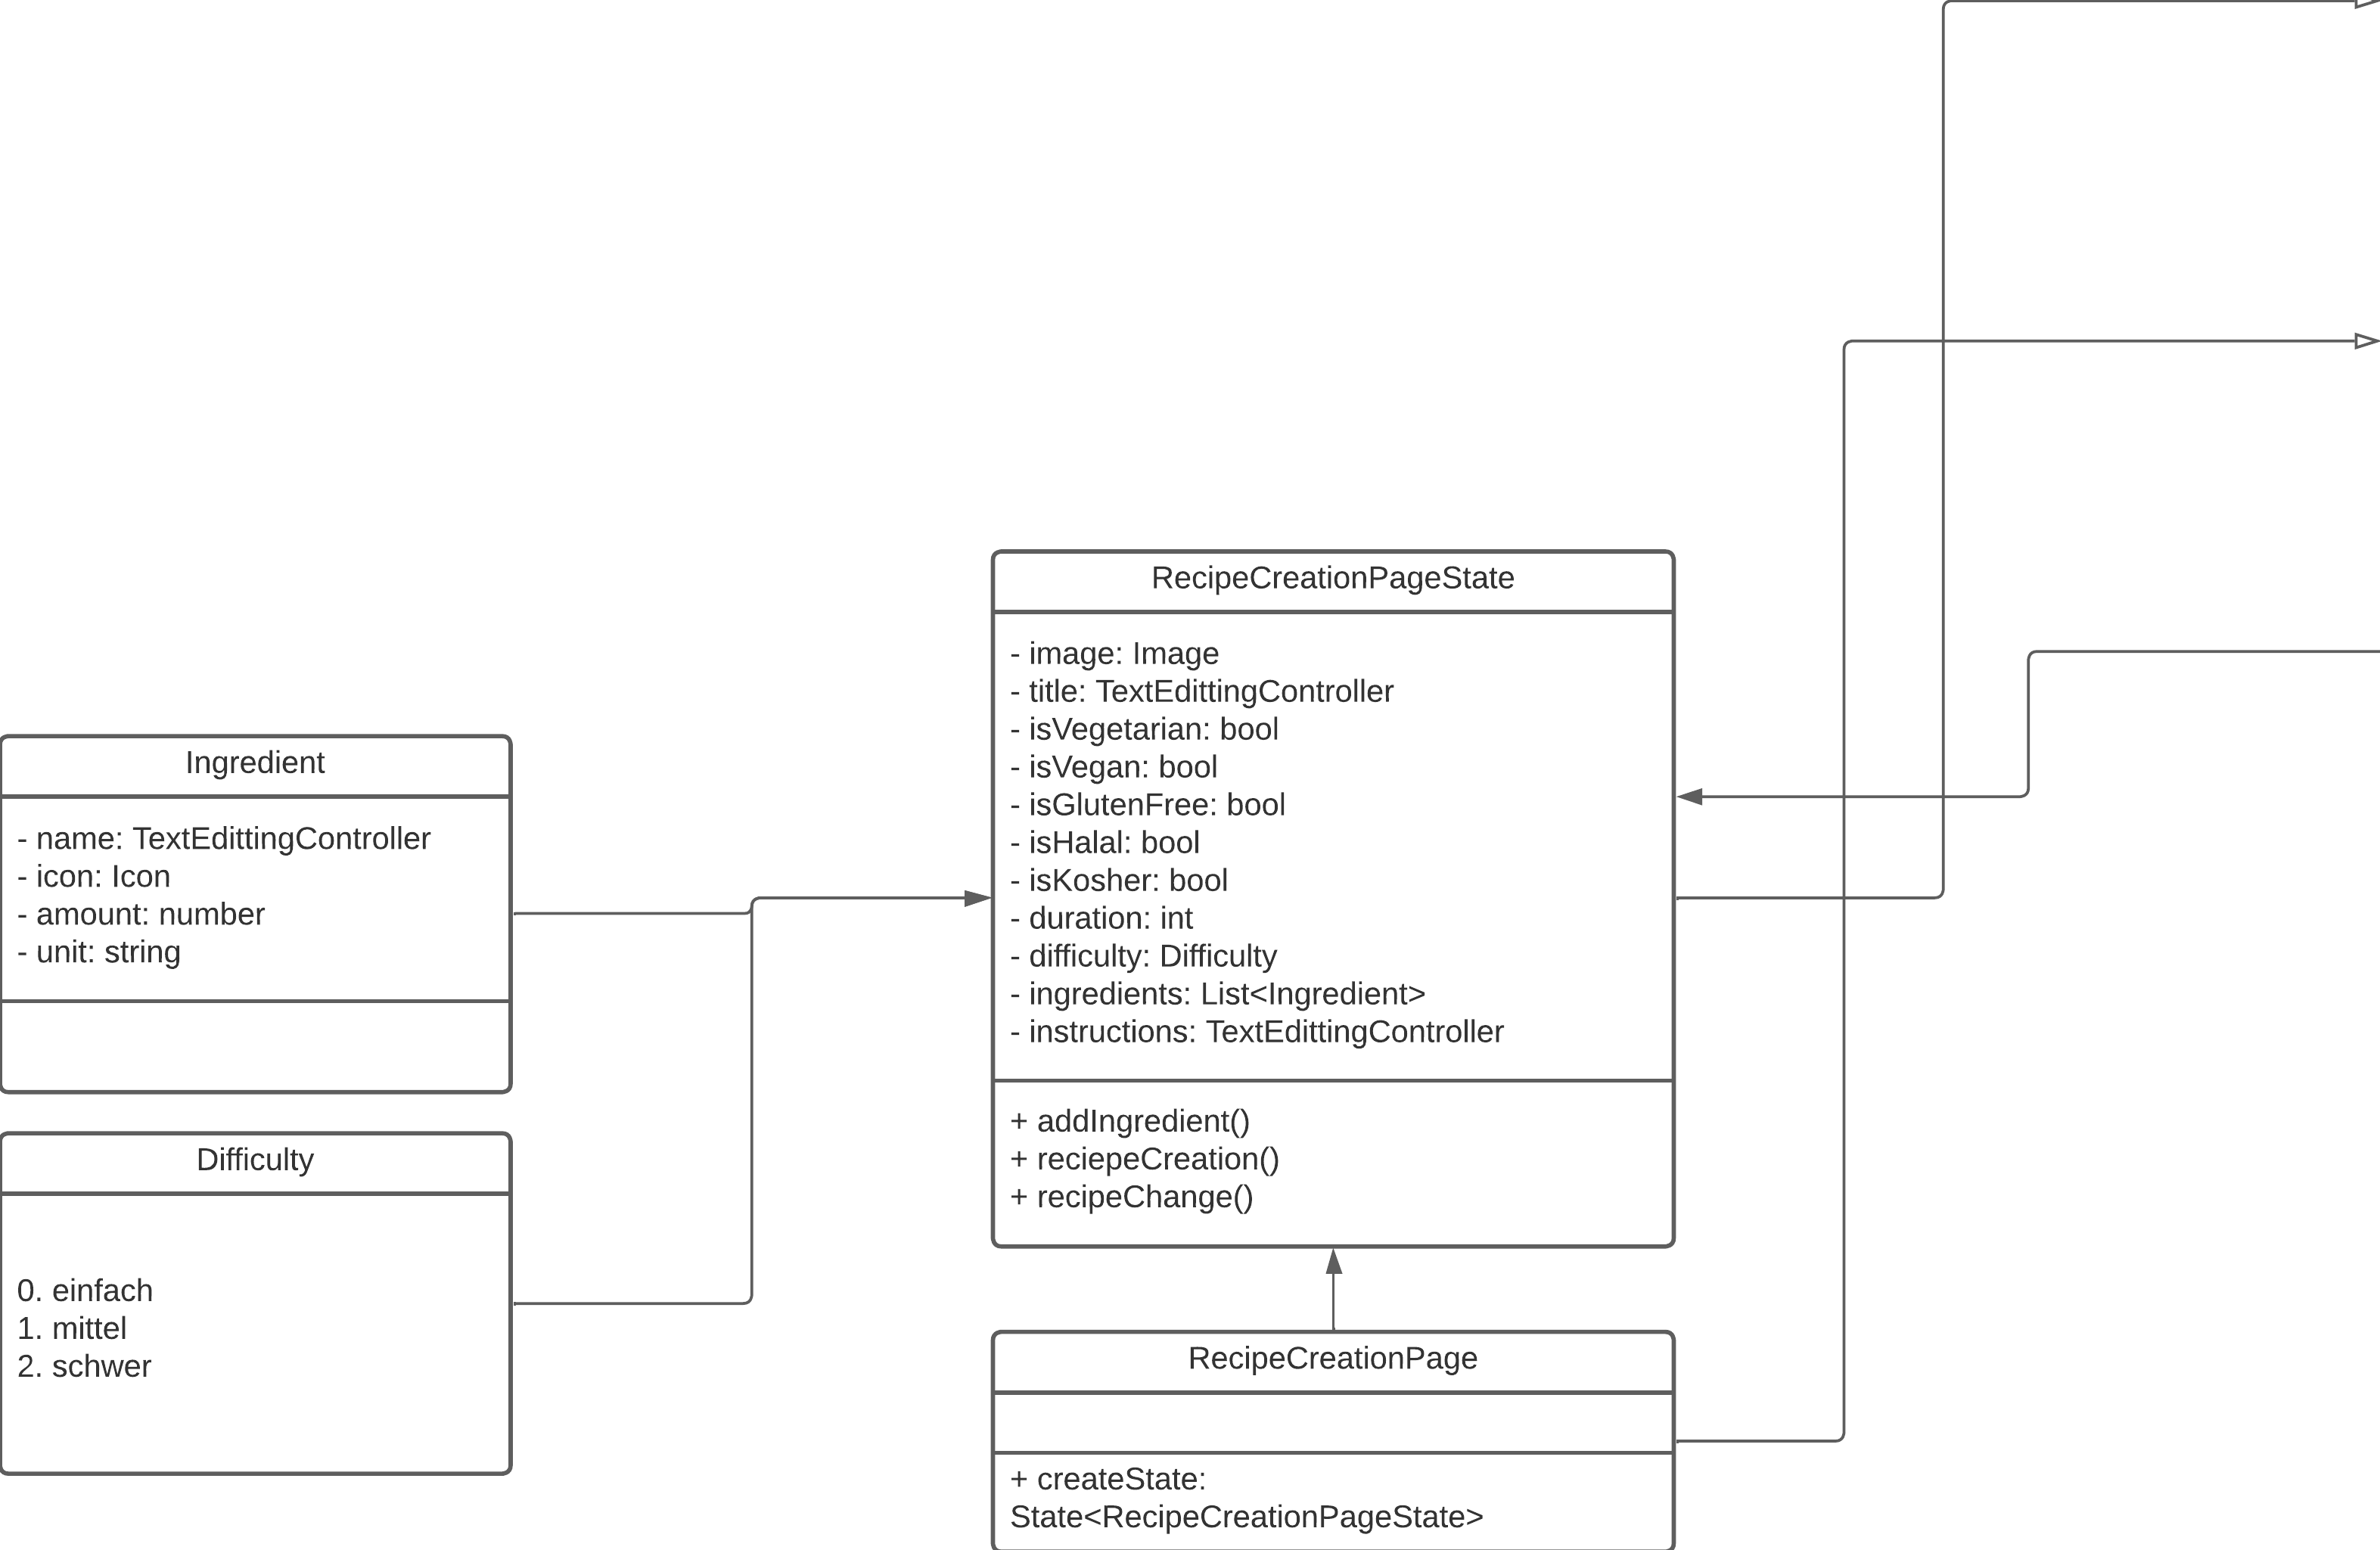
\includegraphics[height = 50mm]{entwurfsheft/images/Presentation-layer/Recipe Creation Page.png}
        %        \caption{RecipeCreationPage}
        %    \end{minipage}
        %\end{figure}

        \newpage
        
        \subsection{Add Ingeredient Page}
            Die Klassen beinhaltet alle nötigen Funktionen und Attribute um die Zutaten-Auswahl-Ansicht darzustellen.\newline
        \textbf{Attributes}
        \begin{itemize}
            \item ingredient: Die Ausgewählten Daten zur Datstellung einer Zutat.
        \end{itemize}
        
        \textbf{Methods}
        \begin{itemize}
            \item addIngerdient(ingerdient: Ingeredient): Fügt dem Rezept eine neue Zutat hinzu. 
        \end{itemize}
        
            \subsubsection{Ingeredient}
                Die Klasse stellt eine Zutat für eine Rezept da.
                \textbf{Attributes}
                    \begin{itemize}
                        \item name: Die eingegebene Zeichenkette für den Namen der Zutat.
                        \item iconId: Die ID des ausgewählten Icons.
                        \item amount: Die ausgewählte Anzahl der Zutat für das Rezept.
                        \item unit: Die Einheit in der die Zutat bemessen wird.
                    \end{itemize}
                    
                \textbf{Methods}
                    \begin{itemize}
                        \item choseIcon(iconId: String): Fügt der Zutat eine Icon hinzu. 
                    \end{itemize}

        \newpage
        
         \subsection{Groupe Detail Page}
            Die Klassen beinhaltet alle nötigen Funktionen und Attribute um die Gruppen-Detail-Ansicht darzustellen.\newline
            
        \subsubsection{GroupeDetailPageState}
            \textbf{Methods}
            \begin{itemize}
                \item changeGroupeName(name: String): Ändert den Gruppennamen auf die eingegbene Zeichenkette.
                \item leaveGroup(userId: string): Der User ist nicht mehr teil der Gruppe.
                \item deleteGroup(userId: string): Die Gruppe wird gelöscht und dabei werden alle Mitgleider entfernt.
                \item getQRCode(userId: string): Der QR-Code zum Beitretten der Gruppe wird erstellt und bereitgestellt.
                \item getGroupId(userId: string): Die Gruppen ID wird ausgegeben.
                \item kickUser(userId: string): Der User mit der angegeben ID wird aus der Gruppe entfernt.
                \item banUser(userId: string): Der User mit der angegeben ID wird aus der Gruppe entfernt, auf eine Blacklist gesetzt sodass er nicht mehr beitretten kann.
                \item makeAdmin(userId: string): Der User mit der angegeben ID wird zu einem Admin der Gruppe.
                \item removeAdminStatus(userId: string): Der User mit der angegeben ID wird der Adminstatus entfernt.
                \item togglePrivate(recipeId: string): Für das Rezeot mit der angegeben ID wird die \gls{sichtbarkeit} geändert.
            \end{itemize}

        \subsubsection{GroupeDetailPage}
            \textbf{Methods}
            \begin{itemize}
                \item createState: State<GroupeDetailPageState>: Erstellt einen GroupeDetailPageState.
            \end{itemize}

        \subsubsection{GroupeWidget}
            \textbf{Methods}
            \begin{itemize}
                \item delete(): 
                \item change()
                \item togglePrivate()
            \end{itemize}

        \subsubsection{GroupeDUserWidget}
            \textbf{Attributes}
            \begin{itemize}
                \item ownAccount: Gibt an ob es sich bei dem dargsetellten User um den eigenen Account handelt.
            \end{itemize}
            
            \textbf{Methods}
            \begin{itemize}
                \item  Mitgliedelement(required isOwnAccount: bool):
                \item  kickUser(di: String):
                \item  banUser()
                \item  makeAdmin()
                \item  removeAdminStatus()
            \end{itemize}
    
        \newpage
        
         \subsection{Groupe Detail Page}
            Die Klassen beinhaltet alle nötigen Funktionen und Attribute um die  darzustellen.\newline
        \textbf{Attributes}
        \begin{itemize}
            \item 
        \end{itemize}
        
        \textbf{Methods}
        \begin{itemize}
            \item 
        \end{itemize}
 
\newpage
\section{Glossar}
\printglossary[style=altlist]
\end{document}